% Chapter Template

\chapter{Implementation} % Main chapter title

\label{Chapter5} % Change X to a consecutive number; for referencing this chapter elsewhere, use \ref{ChapterX}
%----------------------------------------------------------------------------------------
%	SECTION 1
%----------------------------------------------------------------------------------------
\section{Static Graph Analysis}
\subsection{SMAUG}

We first describe the simulation and compiler framework we work with in order
to show how tensors and mappings are obtained. SMAUG \cite{smaug} is an end to
end full stack simulation framework for deep learning work loads. As an
end-to-end framework SMAUG allows for a high level DSL to be used in order to
describe a model so that many deep learning architectures can be evaluated very
quickly. Further, SMAUG leverages the gem5-Aladdin \cite{aladdin} simulation
framework to describe custom hardware architectures, easily change their
configurations, all without the need for a dedicated backend compiler for each
custom architecture. This allows researchers to iterate and evaluate on many
deep learning workloads, and tune every layer of the stack without the need for
RTL design and laborious backed integrations. To the best of our knowledge, no
other simulation framework allows for the accurate performance analysis and
provides end-to-end configuration support.
\begin{figure}[thb!]
\centering
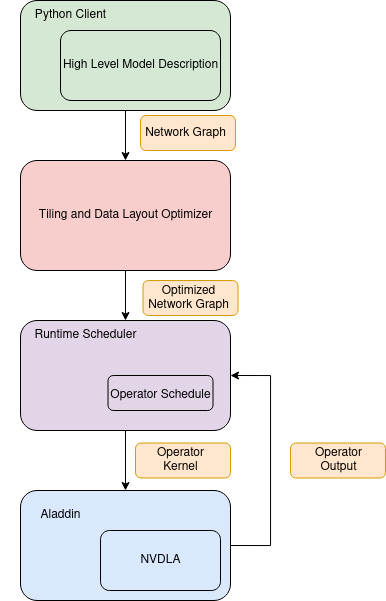
\includegraphics[scale=0.7]{Figures/smaug_stack.png}
\decoRule
\caption[Overview of SMAUG]{Overview of SMAUG framework stack}
\label{fig:SmaugStack}
\end{figure}


From SMAUG we can understand the amount of time and cycles being spent on compute time
over DMA transfers. Different deep learning models call for different operators that
result in diverse levels of memory and compute boundedness. Being able to
analyze operator level differences in DMA and compute times allow us to weight tensors
more heavily towards memory bound operations in the final ILP model.

\lstinputlisting[language=Python, caption={Model
description example},label={lst:minerva_model_desc}, basicstyle=\ttfamily\scriptsize]{Figures/minerva_network.py}


SMAUG is divided into a Python front end used to describe DL topologies, a
runtime middle end that handles execution, and a backend of kernels. An overview
of these parts are shown in figure \ref{fig:SmaugStack}. Models are
created using Python APIs that describe what operations, hardware
configuration, weights and input data, and which set of acerbated kernels a
user wants to use. The front end takes this model description and serialized it
into a form the runtime can read and create an execution context around. The
runtime takes the serialized model description and creates a computation graph.
Example code of a Minerva model description for SMAUG is show in listing
\ref{lst:minerva_model_desc}. The graph is used to perform tiling
optimizations and an operator schedule. Once an operator schedule is created,
the runtime executes each operation sequentially by dispatching each operation
as previous operator outputs are received back into main memory. The backend
contains all the accelerator kernels and are invoked every time the runtime
dispatches an operator. Kernels can be either written in native gem5 or using
Aladdin.
% TODO: figure of framework stack
% TODO: figure of a model description

% TODO: explain how backends are invoked and how hardware is described and configured
% TODO: explain the pipeline of tracing -> simulation for data gathering

\subsection{Static Analysis}

\begin{figure}[thb!]
\centering
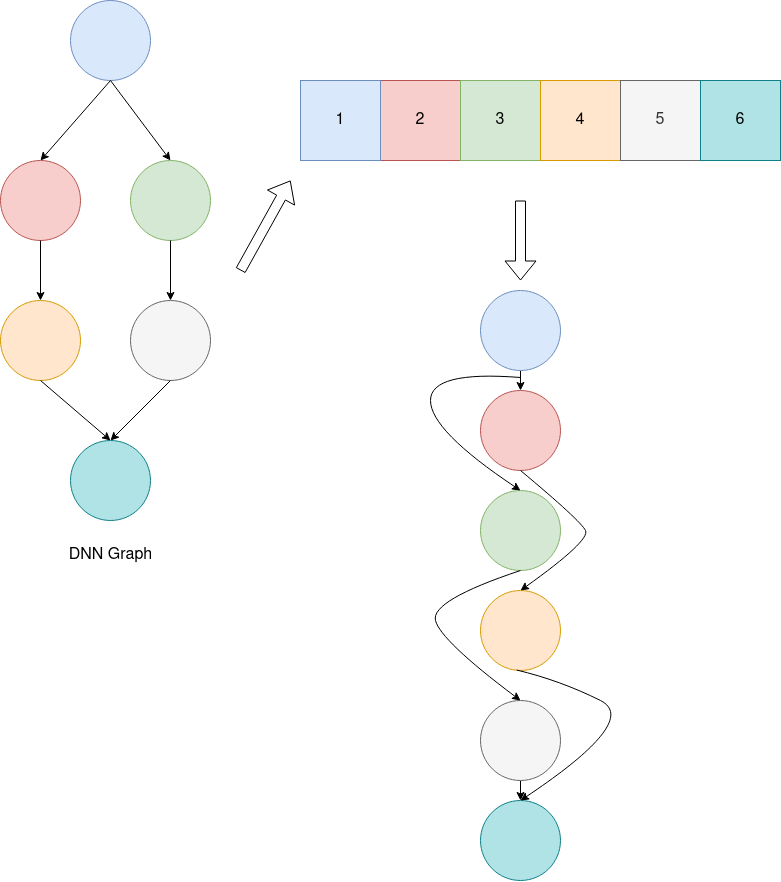
\includegraphics[scale=0.6]{Figures/graph_to_schedule.png}
\decoRule
\caption[Computational Graph to Schedule Conversion]{Illustration of a DNN graph being converted to a schedule}
\label{fig:graphToSchedule}
\end{figure}

Like OnSRAM, we use the computational graph provided by the SMAUG runtime
implemented in C++ to run our static analysis on tensors to devise a SPM
management framework. We allow SMAUG to apply its optimizations and graph
preprocessing to create a final operator schedule. This schedule is what we use
to analyze operator data dependencies and tensor meta information.  Figure
\ref{fig:graphToSchedule} shows how a DNN graph is converted into a schedule
where each node has a sequence number in the schedule. The schedule can be
visualized a new graph where nodes flow down sequentially in schedule order and
vertices show data dependencies. In SMAUG, each operation is represented as a
class has a list of associated input tensors, a list of output tensors, and
what computation the operation requires.  Each tensor is also represented as a
class that holds relevant information such as tensor size, dimensions, and
dimension layout.


% dict of inputs nad outputs per op for a scheudle list enumerate operations in
% the scheudle and create a mapping of a paritcular operation to the sequence
% number in the execution schedule

% create list of unique tensors
% create map of unique tensor to a unique tensor #

% create list of tensor size indexed by tensor #

% create map of tensor # to opreations sequence #'s its used in. The first element is the 
% operation # in which it is created and the last operation # is the final operation it is used in

We iterate through the schedule of operators and create a map where an
operation name is mapped to its sequence number in the operator schedule
For each operator we encounter for each iteration
of the schedule, we take note of the operators input and output tensors. These inputs
and outputs are used to create an array of unique tensors. This array of
tensors is then used to create a mapping of each tensor to a tensor number
where every tensor number is the index of the tensor in the array. A map of 
tensor numbers to the corresponding tensor size is also created. We then
build a map of tensor numbers to an array of operation sequence numbers they are
required in where the first element of the array represents the operation that
the tensor is created and the last element represents the final operation
it is used in.

%TODO: figure of graph -> operator schedule -> data reuse graph



\begin{figure}[thb!]
\centering
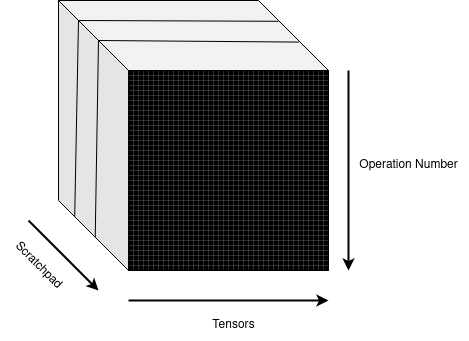
\includegraphics[scale=0.7]{Figures/mapping_matrix_cube.png}
\decoRule
\caption[3D Tensor Mapping Matrix]{Illustration of mapping matrix}
\label{fig:mappingCube}
\end{figure}


\begin{figure}[thb!]
\centering
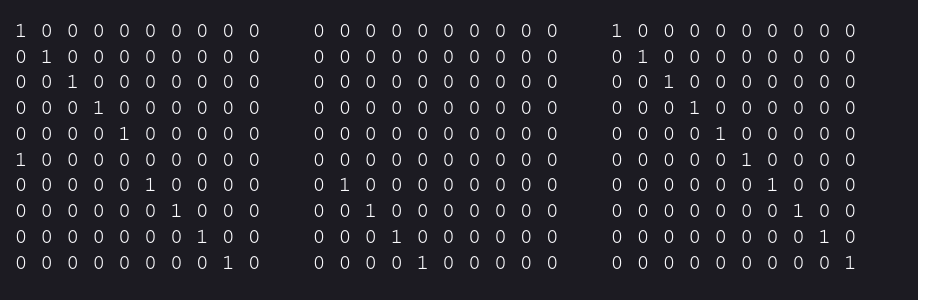
\includegraphics[scale=0.5]{Figures/naive_matrix_mapping.png}
\decoRule
\caption[2D Tensor Mapping Matrix]{Naive SPM mapping matrix representation as an input to the ILP solver}
\label{fig:naiveSPM2D}
\end{figure}

\subsection{SPM Mapping Representation}

The way an SPM mapping is represented is a three dimensional array in which one
dimension represents time i.e the operation sequence number, another represents
the unique tensors, and the final dimension represents what scratchpad they
belong to. Using the dimensions we can show the relationship between what tensor
is mapped to what SPM during what operation. We build such a matrix after the
static analysis phase to formulate an initial naive SPM mapping representation
that would be executed by default on SMAUG. Figure \ref{fig:naiveSPM2D}
illustrates in two dimensions the resulting naive SPM mapping matrix.

% TODO: remake the matrix cube where we blow up a element to show a tensor and
% like a mapping to the grpah or something
%----------------------------------------------------------------------------------------
%	SECTION 2
%----------------------------------------------------------------------------------------
\section{Model Formulation}

We now describe our ILP model to solve the SPM mapping optimization problem. The goal is to minimize
the amount of cost weighted data transfers as much as possible by pinning as many re-usable tensors
as possible. As described in the previous section, we can breakdown a DNN graph into the following variables.

% describe how we structure our matrix
% data trasnfers costs are proportional the size of the tensor being transported because of the limited bandwidth of hte bus, therefore
% tensors with larger sizes will be weighted as a higher cost. The overall transfer itself can be modelled as data entering the SPM and being
% offloaded from the SPM to main memory. This is done by represneting whether a tensor is on teh SPM with a binary variable: 0 for the tensor is in main
% memory and 1 to represnte hte tensor is in the SPM. A tensor being loaded into the SPM from main memory is modelled as a 0 to 1 in the tenosr column. 
% A tensor being saved to main memory is modelled as 1 to 0 in teh tensor time column x[m][k][n] = 1 x[m+1][k][n] = 0

There exists a set of tensors required as inputs and outputs per operation and a unique list of tensors can be constructed.\\
\\
Let $N \coloneqq \{ n \text{ }  | \text{ } n   \text{ represents a tensor ID used in the DNN graph}\}$\\

For each DLA architecture, there exists at least 1 scratchpad with a corresponding size. To refer to each scratchpad and its size on the DLA:\\
\\
Let $K \coloneqq \{ k \text{ }  | \text{ } k   \text{ represents a scratchpad ID}\}$\\
Let $Q \coloneqq \{ q \text{ }| \text{ } \text{where } Q_k \text{ represents the size of Scratchpad$_k \in K$}\}$\\

Once a graph has been scheduled, each operation can be referenced by its sequence number.\\
\\
Let $M \coloneqq \{ m \text{ }  | \text{ } m   \text{ represents an operation in the DNN graph}\}$\\

Due to limited bus bandwidth, tensors with different sizes will require
different amounts of DMA transfers proportional to their size. In order to keep
track of the sizes so that we can weight each tensor with a certain cost:\\
\\
Let $S \coloneqq \{ s \text{ }| \text{ } \text{where } S_n \text{ represents the size of tensor$_n \in N$}\}$\\


So the mapping matrix can be described as a three dimensional matrix where every position is a binary variable such that\\
\\
$x[n][k][m] \in \{0, 1\} \forall n,k,m $\\
$x[n][k][m] = 1$ represents a tensor $n$ that occupies scratchpad $k$ at operation $m$ \\
$x[n][k][m] = 0$ represents a tensor $n$ does not exist on scratchpad $k$ at operation $m$\\

If $x[n][k][m] = 0 \forall k$ then it means that tensor $n$ is saved to main memory at operation $m$.


\subsection{Objective Function}
The objective function we would like to solve for such that we minimize the
amount of cost weighted data transfers is the following:\\
\\
\[
min(\sum_n \sum_k \sum_m S_n * (|x[n][k][m+1] - x[n][k][m]|))
\]
\\

A difference between $|x[n][k][m+1] - x[n][k][m]|$ represents either a data
transfer of tensor $n$ from SPM $k$ to main memory if $x[n][k][m+1] -
x[n][k][m] = -1$ or main memory to SPM if $x[n][k][m+1] - x[n][k][m] = 1$.
$|x[n][k][m+1] - x[n][k][m]|$ shows that either a tensor $n$ remains on SPM $k$
between operations $m$ and $m+1$ or stays in main memory.

By minimizing the sum of total data transfers multiplied by the tensor size, we
minimize on a cost basis the amount of DMA loads and stores and maximize
tensors being reused on the SPM. However, the absolute value in the objective function
would make it non-linear. Thus, we add auxiliary variables to remove the absolute values
and reformulate the objective function as:\\
\\
\[
min(\sum_n \sum_k \sum_m y[n][k][m])
\]

\subsection{Constraints}
We now describe the following set of constraints on the model:
\begin{itemize}
	\item All necessary input and output tensors for a given operation will be present on the SPMs\\

		Let $A \coloneqq \{ a \text{ } | \text{ } \text{where } A[n] = 1\text{ represents a tensor$_n$ is required as an input or output for operation$_m$} \}$\\
		\[
			A[n][m] \in \{0, 1\} \forall n,m
		\]

		\[
			A[n][m] = 1 \implies \sum_{i \in K} x[n][i][m] = 1 
		\]

	\item All tensors mapped on an SPM$_k$ must fit on within the given scratchpad space\\

		$\sum_{i \in N} {x[i][k][m] * s[i]} \leq Q[k] \forall m,k$\\

	\item Tensors are not mapped before the operation in which they're lifetime begins \\

		Let $B \coloneqq \{ b_n \text{ } | \text{ }  b_n \text{represents the start time for tensor $n$}\}$ \\

		$x[n][m][k] = 0 \forall m < B_m$

	\item Tensors are not mapped after the operation in which they're lifetime ends \\

		Let $E \coloneqq \{ e_n \text{ } | \text{ }  e_n \text{represents time for tensor $n$}\}$ \\

		$x[n][m][k]= 0 \forall m > E_m$

	\item Absolute Value Constraints\\
		Let $Y = \{ y[0][0][0], y[0][0][1], ... y[n][k][m]\prime\}$\\
		$(x[n][k][m+1] - x[n][k][m]) * S_n <= y[n][k][m]$\\
		$(x[n][k][m] - x[n][k][m + 1]) * S_n <= y[n][k][m]$\\

\end{itemize}

\subsection{Solver}
This model description can now be used to find the exact solution to the SPM
mapping problem. We use the Gurobi ILP solver and the Python API to create our
optimized mapping matrix. The listed constraints can be used as is and the
original $X$ variable is initialized with the naive mapping matrix.  An
illustration of the optimized matrix is show in figure \ref{fig:optimalSPM2D}.
This new matrix can be used to integrate a pinning strategy in the framework.

\begin{figure}[thb!]
\centering
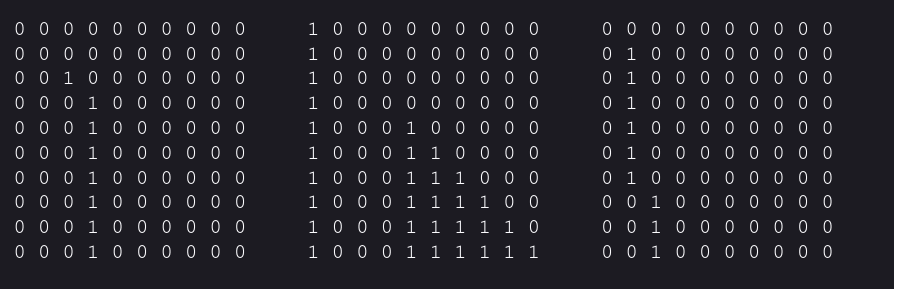
\includegraphics[scale=0.55]{Figures/optimal_matrix_mapping.png}
\decoRule
\caption[Optimal Mapping 2D Matrix]{Optimal SPM mapping matrix representation as an input to the ILP solver}
\label{fig:optimalSPM2D}
\end{figure}

